
\documentclass{article}

\usepackage[utf8]{inputenc}

\usepackage{amsmath, bm}
\usepackage{graphicx}
\usepackage{amssymb}
\usepackage{float}
\usepackage{caption}
\usepackage{subcaption}
\usepackage{hyperref}
\usepackage{tikz}
\usepackage{layout}

\usepackage[margin=1in]{geometry}
\usepackage{listings}
\usepackage{xcolor}
\usepackage{color, colortbl}
\usepackage{textgreek}
\usepackage{mathrsfs}
\usepackage{savetrees}

\usepackage{titlesec}

\titleformat{\subsubsection}
  {\normalfont\selectfont}{\thesubsubsection}{1em}{}

\usetikzlibrary{calc}
\usetikzlibrary{angles,quotes} % for pic
\usetikzlibrary{patterns,snakes}
\usetikzlibrary{arrows}
\tikzset{>=latex} % for LaTeX arrow head

\setlength{\parskip}{\baselineskip}%
\setlength{\parindent}{0pt}%
\linespread{0.9}


\definecolor{codegreen}{rgb}{0,0.6,0}
\definecolor{codegray}{rgb}{0.5,0.5,0.5}
\definecolor{codepurple}{rgb}{0.58,0,0.82}
\definecolor{backcolour}{rgb}{0.95,0.95,0.92}

\lstdefinestyle{mystyle}{
    backgroundcolor=\color{backcolour},   
    commentstyle=\color{codegreen},
    keywordstyle=\color{magenta},
    numberstyle=\tiny\color{codegray},
    stringstyle=\color{codepurple},
    basicstyle=\ttfamily\footnotesize,
    breakatwhitespace=false,         
    breaklines=true,                 
    captionpos=b,                    
    keepspaces=true,                 
    numbers=left,                    
    numbersep=5pt,                  
    showspaces=false,                
    showstringspaces=false,
    showtabs=false,                  
    tabsize=2
}

\lstset{style=mystyle}


\begin{document}

\title{}
\author{lwp26}
\date{November 2024}
\maketitle 

\iffalse
\begin{abstract}
    \centering
    LOg bAs
\end{abstract}
\fi

%-----------------------------------------------------------------------------------------
\section{Introduction}
%-----------------------------------------------------------------------------------------

\subsection{Objectives}

\subsection{Setup}

\begin{figure}[H]
    \centering
    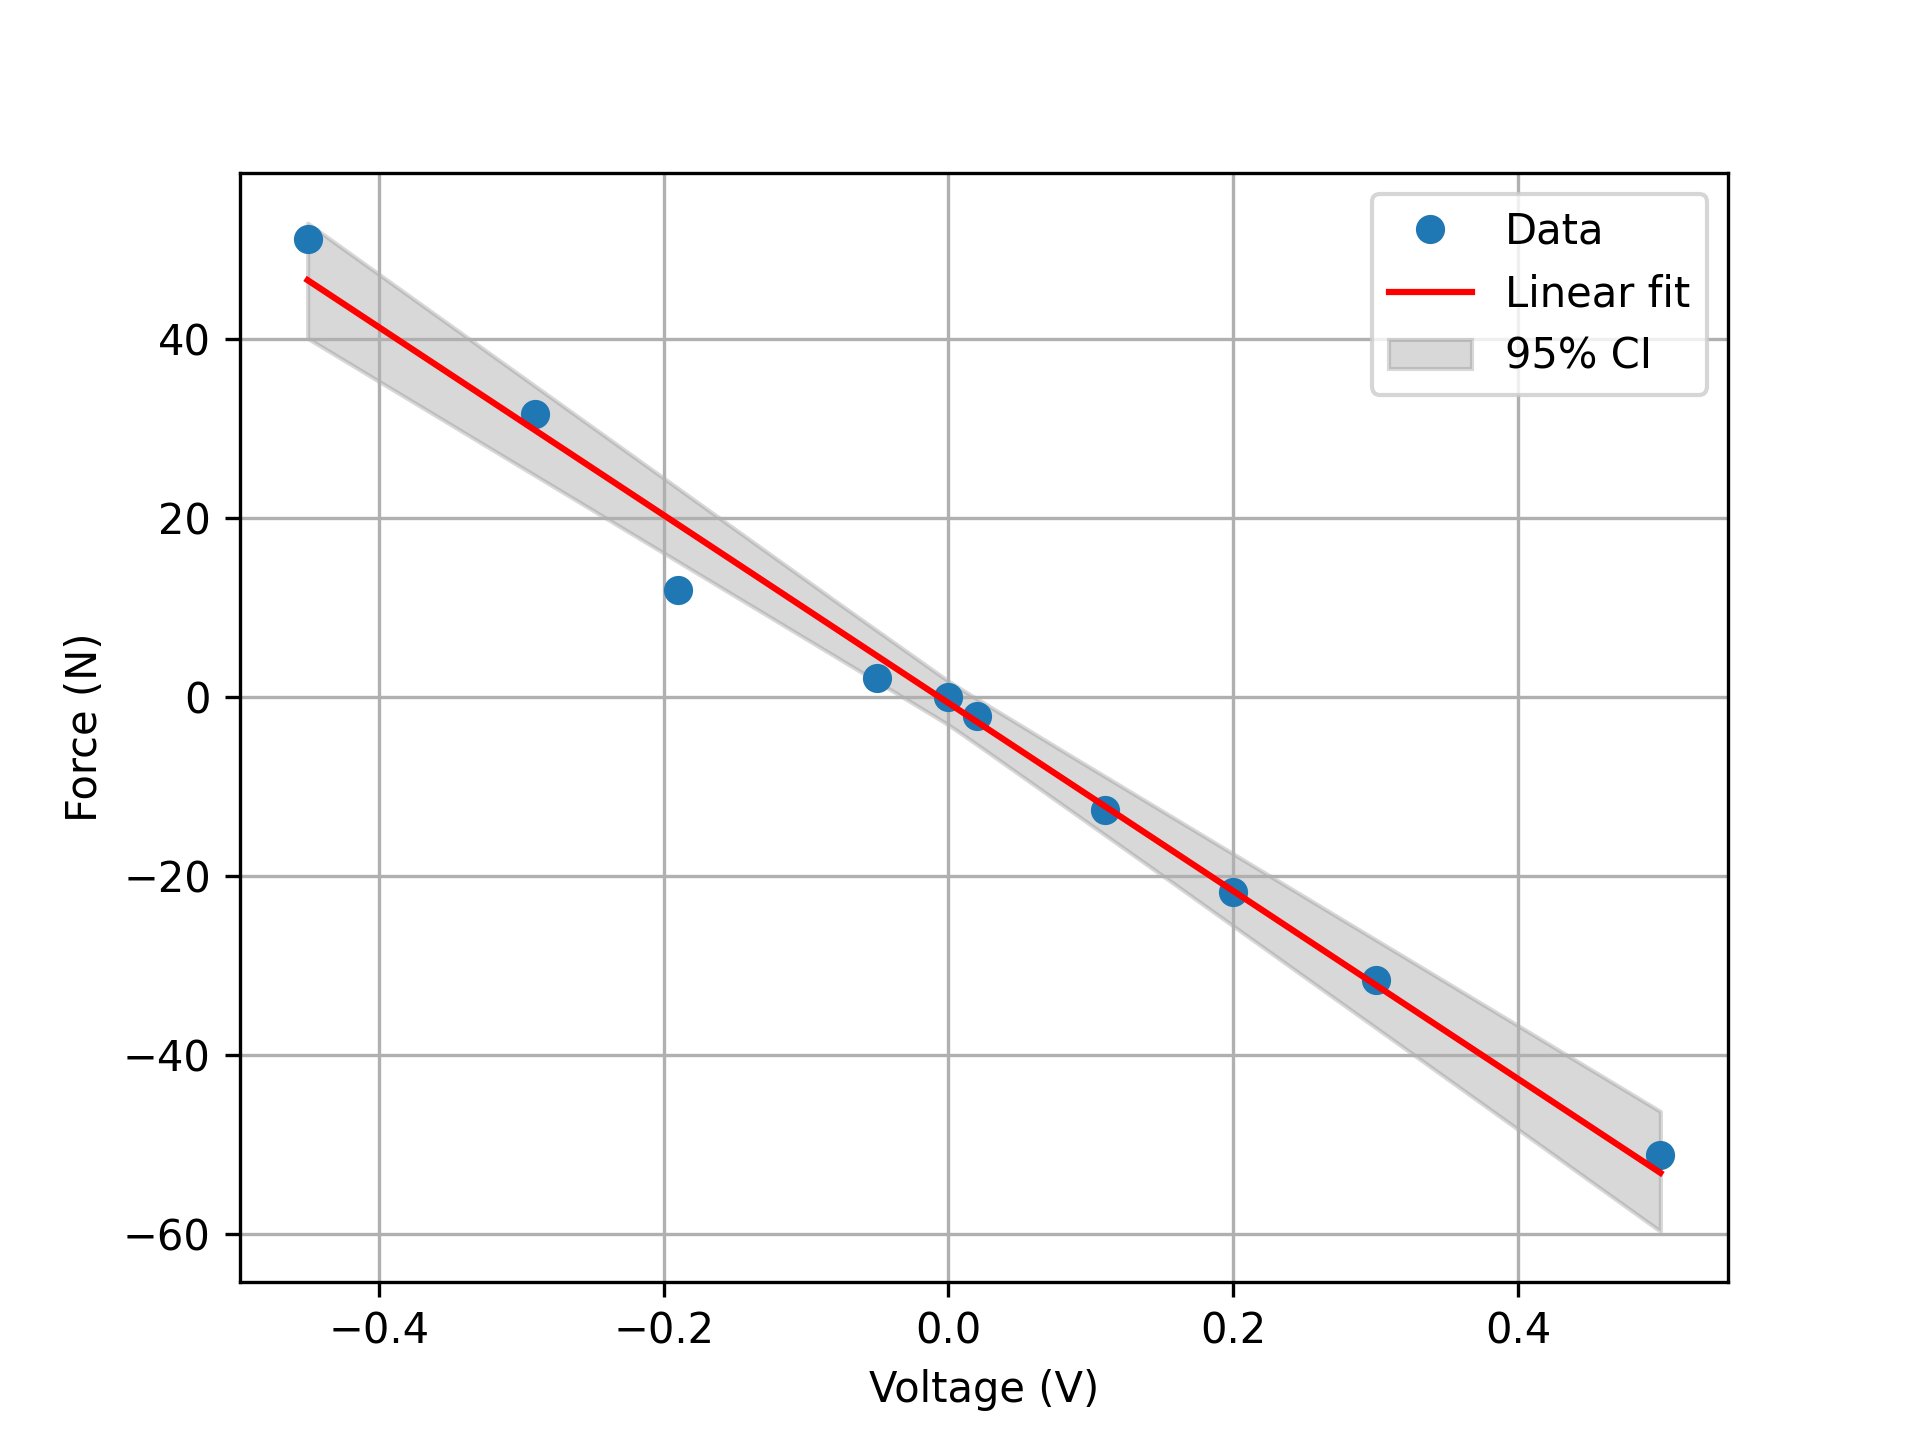
\includegraphics[width=0.8\textwidth]{Calibration/linearity.png}
    \caption{Loss coefficient for various operating Mach and Reynolds numbers.}
    \label{fig:force_linearity}
\end{figure}

\section{LATERAL CREEP}

\subsection{\textbf{Transducer Calibration}}

\begin{center}
    \textbf{Comment on the accuracy and linearity of the side force transducer}
\end{center}

\subsection{\textbf{Effect Of Speed On Side Force}}

\begin{center}
    \textbf{Comment on the influence of rolling speed on the average steady state lateral forces
    developed by the model tyre.}
\end{center}

\subsection{\textbf{Effect of Normal Load on Steady State Side Force}}

\begin{center}
    \textbf{What causes the microslip?}
\end{center}

\begin{center}
    \textbf{Comment on the relationship between the amount of microslip in the contact area and
    the shape of the Y vs. $ \alpha $ graph}
\end{center}

\begin{center}
    \textbf{At which normal load is the tyre nearest to sliding for large
    $ \alpha $ ? Why? How is the
    linear range of Y vs.
    $ \alpha $ affected by the normal load?}
\end{center}

\section{LONGITUDINAL CREEP}

\subsection{\textbf{No Load Creep}}

\subsection{\textbf{Creep with an Applied Torque}}

\begin{center}
    \textbf{ Comment on the longitudinal deformation and compare it with the lateral deformation
    in section 4.3. Where is sliding most likely to occur? Comment also on the
    relationship between the amount of sliding in the contact area and the shape of the X
    vs.
    ξ graph.}
\end{center}



\begin{equation}
    \xi = \frac{\Delta x}{x} 
     = \frac{x_{2} - x_{1}}
            {\bigl(x_{\max} - x_{1}\bigr) + \bigl(x_{\max} - x_{2}\bigr)}.
\end{equation}

\subsection{\textbf{Combined Lateral and Longitudinal Creep}}

\begin{center}
    \textbf{Comment on the comparison between theory and experiment.}
\end{center}

\section{Appendix}

\begin{thebibliography}{9}


  \bibitem{handout}
  J. V. Taylor
  \emph{Turbine Cascade Aerodynamics Handout}
  University of Cambridge,
  October 2024.

  \bibitem{losses}
  J. D. Denton (1993).
  \emph{Loss Mechanisms in Turbomachines}
  May, 1993 

  \bibitem{fluidmech}
  S. L. Dixon
  \emph{Fluid Mechanics, Thermodynamics of Turbomachinery, FOURTH EDITION}
  1998

  \bibitem{separation}
  John M. Russell
  \emph{LENGTH AND BURSTING OF SEPARATION BUBBLES: A PHYSICAL INTERPRETATION}
  1979
\end{thebibliography}

\end{document}